\documentclass[12pt,nohyper]{tufte-handout}\usepackage[]{graphicx}\usepackage[]{color}
%% maxwidth is the original width if it is less than linewidth
%% otherwise use linewidth (to make sure the graphics do not exceed the margin)
\makeatletter
\def\maxwidth{ %
  \ifdim\Gin@nat@width>\linewidth
    \linewidth
  \else
    \Gin@nat@width
  \fi
}
\makeatother

\definecolor{fgcolor}{rgb}{0.345, 0.345, 0.345}
\newcommand{\hlnum}[1]{\textcolor[rgb]{0.686,0.059,0.569}{#1}}%
\newcommand{\hlstr}[1]{\textcolor[rgb]{0.192,0.494,0.8}{#1}}%
\newcommand{\hlcom}[1]{\textcolor[rgb]{0.678,0.584,0.686}{\textit{#1}}}%
\newcommand{\hlopt}[1]{\textcolor[rgb]{0,0,0}{#1}}%
\newcommand{\hlstd}[1]{\textcolor[rgb]{0.345,0.345,0.345}{#1}}%
\newcommand{\hlkwa}[1]{\textcolor[rgb]{0.161,0.373,0.58}{\textbf{#1}}}%
\newcommand{\hlkwb}[1]{\textcolor[rgb]{0.69,0.353,0.396}{#1}}%
\newcommand{\hlkwc}[1]{\textcolor[rgb]{0.333,0.667,0.333}{#1}}%
\newcommand{\hlkwd}[1]{\textcolor[rgb]{0.737,0.353,0.396}{\textbf{#1}}}%

\usepackage{framed}
\makeatletter
\newenvironment{kframe}{%
 \def\at@end@of@kframe{}%
 \ifinner\ifhmode%
  \def\at@end@of@kframe{\end{minipage}}%
  \begin{minipage}{\columnwidth}%
 \fi\fi%
 \def\FrameCommand##1{\hskip\@totalleftmargin \hskip-\fboxsep
 \colorbox{shadecolor}{##1}\hskip-\fboxsep
     % There is no \\@totalrightmargin, so:
     \hskip-\linewidth \hskip-\@totalleftmargin \hskip\columnwidth}%
 \MakeFramed {\advance\hsize-\width
   \@totalleftmargin\z@ \linewidth\hsize
   \@setminipage}}%
 {\par\unskip\endMakeFramed%
 \at@end@of@kframe}
\makeatother

\definecolor{shadecolor}{rgb}{.97, .97, .97}
\definecolor{messagecolor}{rgb}{0, 0, 0}
\definecolor{warningcolor}{rgb}{1, 0, 1}
\definecolor{errorcolor}{rgb}{1, 0, 0}
\newenvironment{knitrout}{}{} % an empty environment to be redefined in TeX

\usepackage{alltt}
\usepackage[T1]{fontenc}
\usepackage[latin9]{inputenc}
\usepackage{wrapfig}
\usepackage{longtable}
\usepackage{hyperref}
\usepackage{graphicx}
\usepackage[space]{grffile}

\makeatletter
\makeatother
\IfFileExists{upquote.sty}{\usepackage{upquote}}{}
\begin{document}



\centerline{\Large\bf Statistics 101 Analysis}
\centerline{\bf Homework Comparison by Topics and Sections}
\centerline{\bf }


\section{Overview}

The report will compare the homework outcomes from 
2 sections in 2 topics.

There are totally 100 students 
who submitted the answers. 
100
of them did all the homeworks. A summary of the number of students
and counts of the missing homeworks are displayed in Table \ref{tab:count}.

Since different homeworks have different full scores, 
the percentages correct are used to compare among homeworks.
The average correct percents for the 4 homeworks are 
shown in Table \ref{tab:mean}.

Figure \ref{mar:line} shows the temporal change of students' performance,
and Figure \ref{fig:hist} compares the histograms of those homeworks.

\begin{marginfigure}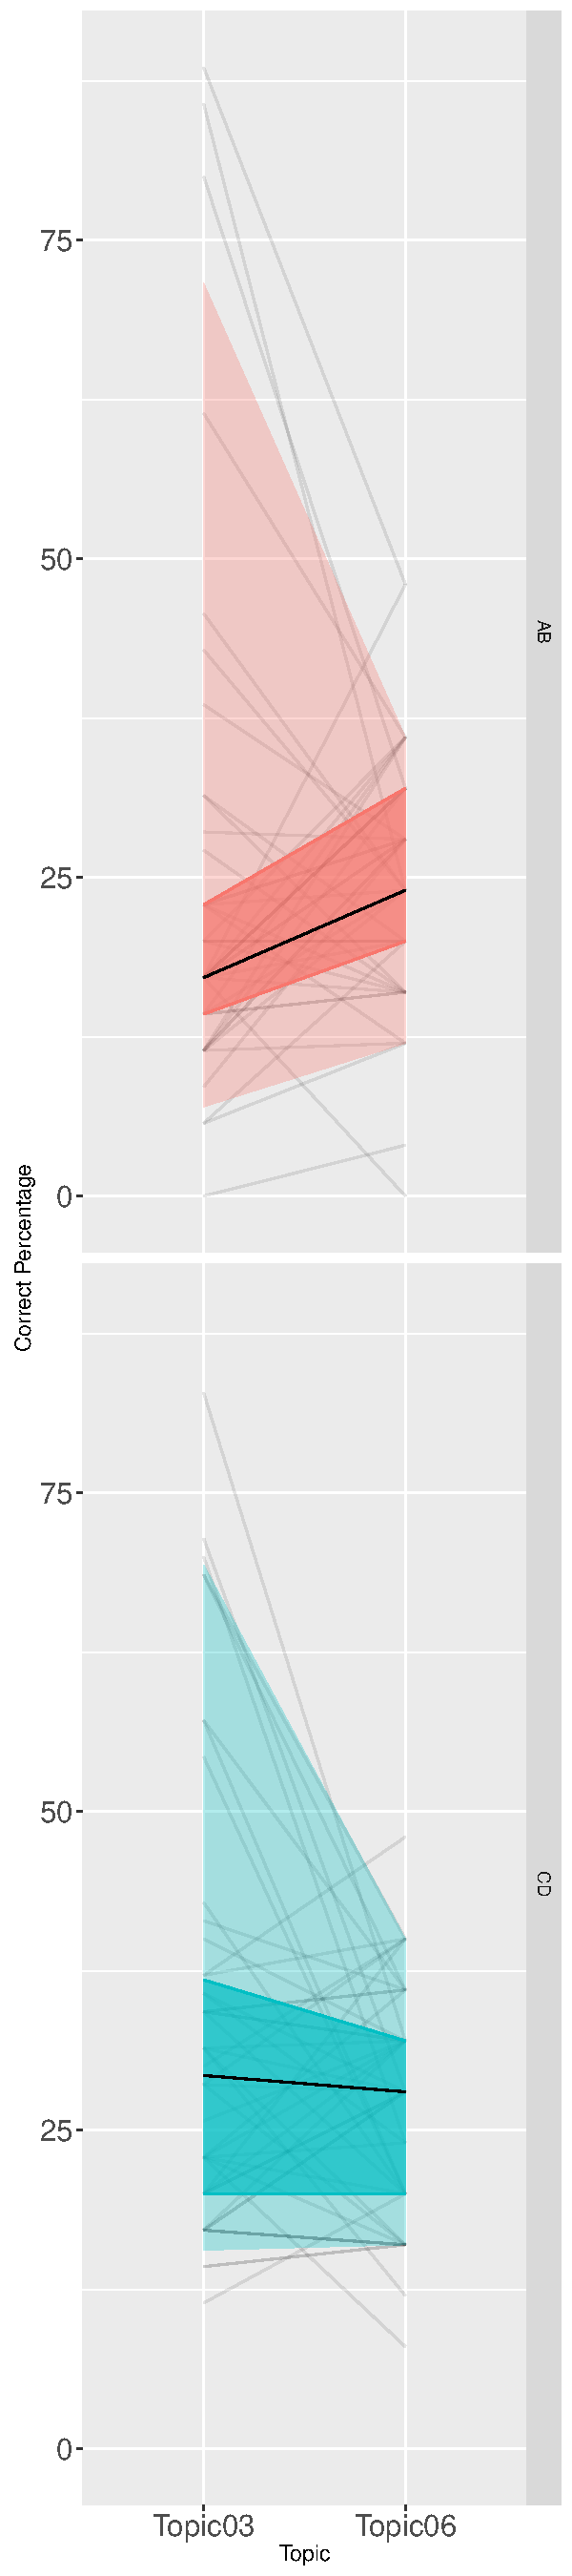
\includegraphics[width=0.95\linewidth]{Stat101_allSections_lineplot}
\caption{\label{mar:line}Line plots of the correct percentages by section.
The black lines give the medians in each topic;
the dark colored areas show the interquartile ranges(25\%-75\%);
and the light colored areas are the 5\%-95\% bands.
The light grey lines are the real correct percentage by student.}
\end{marginfigure}% latex table generated in R 3.2.2 by xtable 1.8-0 package
% Sat Jan 16 13:50:55 2016
\begin{longtable}{rrrr}
  \hline
 & Total & Missing.Topic03 & Missing.Topic06 \\ 
  \hline
AB &  50 &   0 &   0 \\ 
  CD &  50 &   0 &   0 \\ 
   \hline
\hline
\caption{The number of students and counts of missing 
                      homeworks by section. The first column is the number 
                      of students, and the rest columns are the number of 
                      missing homeworks.} 
\label{tab:count}
\end{longtable}
% latex table generated in R 3.2.2 by xtable 1.8-0 package
% Sat Jan 16 13:50:55 2016
\begin{longtable}{rrr}
  \hline
 & Topic03 & Topic06 \\ 
  \hline
AB & 23.80 & 24.96 \\ 
  CD & 32.71 & 27.04 \\ 
   \hline
\hline
\caption{Average correct percentages by section and topic.} 
\label{tab:mean}
\end{longtable}
\begin{center}
\begin{wrapfigure}{o}{1.25\columnwidth}
\begin{centering}
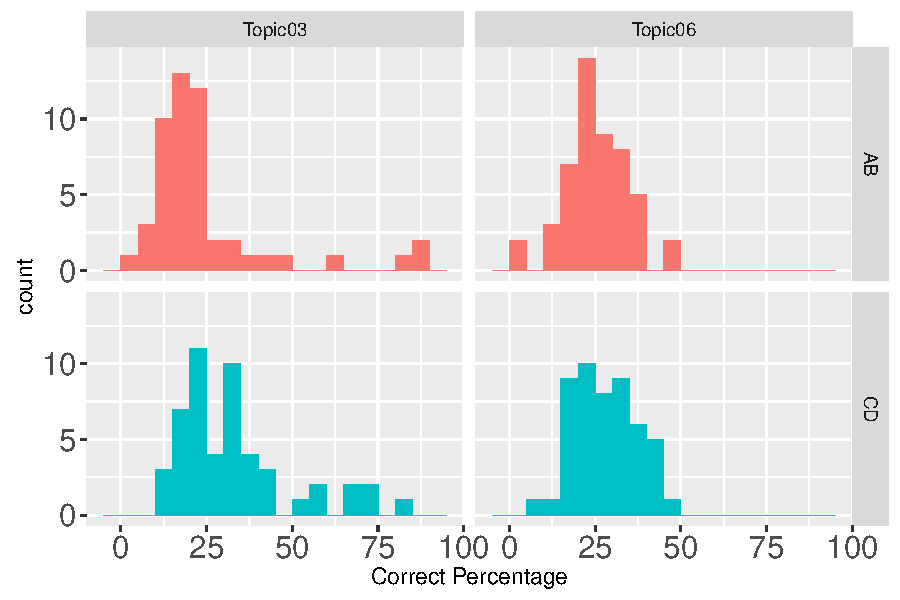
\includegraphics[width=0.95\linewidth]{Stat101_allSections_histbystu}
\par\end{centering}
\caption{\label{fig:hist}Histograms of the percentages correct by section and topic.}
\end{wrapfigure}\par\end{center}

\clearpage
\newpage{}
\section{Factor effects and comparisons}



To analyze the effects of sections and topics on students' performance, 
we consider the generalized linear mixed model, with the response 
(homework score), and the predictors 
(section and topic).

Let $Y_{ijk}$ denote the score that the $k$th student in Section 
$j$ gets for Topic $i$. $i=1,...,$2 topics; 
$j=1,...,$2 sections; $k=1,...,n_j$ students.

Consider that most homework questions give 1 point for 1 correct 
answer, for example, a multiple choice is usually 1 point;
a matching question with 6 items is usually 6 points.
Hence we assume that the full point is equal to the number of 
questions in one homework, and the students can only get 
either 0 or 1 point for each question. Assume that the correct 
probabilities of the questions in one homework are homogeneous, 
denoted by $p_{ijk} \in (0,1)$, then we have 
\[
Y_{ijk} \sim Binomial(N_i, p_{ijk})
\]
where $N_i$ is the full point (i.e., the total number of questions) 
of the $i$th homework.

A mixed effects model is considered since we have 
multiple measurements on each student, while the students 
may have different ability to study. The fixed effects are 
topic ($t$), section ($s$), and their interaction ($ts$). The 
random effect is student ($u$). 

Note that 100 students are divided into 
2 sections. One issue is that 
if we believe $\sigma_{u}^{2}$ are equal between 
the sections. In this study we assume that the variances of 
random effects are not equal, i.e., $u_{jk} \sim N(0,\sigma_{j}^{2})$.
Hence we have the following equation,
\[
g(p_{ijk}) = \mu + t_{i}+s_{j}+ts_{ij}+u_{jk}
\]
where $g()$ is the link function. By default the software R will
set $t_{1}=0$, $s_{1}=0$ and $ts_{ij}=0, \forall i,j = 1 $ 
as the identifiability constraints.

%The result for the fixed effects is in Table \ref{tab:model}. 
%The asterisks indicates the significant coefficients at the 0.05 $\alpha$-level.
The result of the model is as below. Figure \ref{mar:fitted} compares 
the fitted values with the response. Figure \ref{fig:est_sec} 
shows the estimated correct probability.
\begin{marginfigure}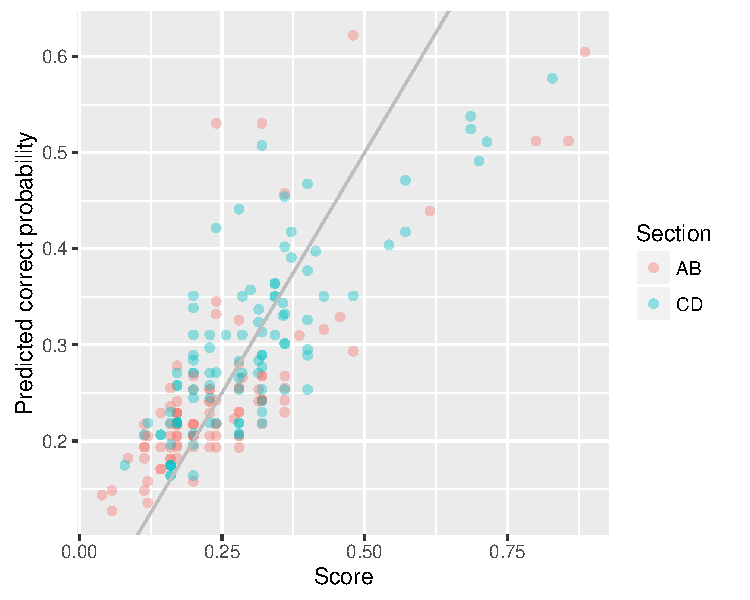
\includegraphics[width=0.95\linewidth]{Stat101_allSections_fitted}
\caption{\label{mar:fitted}Scatterplot between the scaled scores and the 
predicted correct probability. The predicted probability is continuous in (0,1).
But the true scores are discrete.}
\end{marginfigure}
\clearpage
\begin{knitrout}
\definecolor{shadecolor}{rgb}{0.969, 0.969, 0.969}\color{fgcolor}\begin{kframe}
\begin{verbatim}
## Generalized linear mixed model fit by maximum likelihood (Adaptive
##   Gauss-Hermite Quadrature, nAGQ = 0) [glmerMod]
##  Family: binomial  ( logit )
## Formula: Score ~ Topic * Section + (1 | Student)
##    Data: score
## Weights: FullPoints
## 
##      AIC      BIC   logLik deviance df.resid 
##   1140.2   1156.6   -565.1   1130.2      193 
## 
## Scaled residuals: 
##     Min      1Q  Median      3Q     Max 
## -2.9101 -0.7511 -0.1837  0.5946  4.0839 
## 
## Random effects:
##  Groups  Name        Variance Std.Dev.
##  Student (Intercept) 0.2579   0.5078  
## Number of obs: 198, groups:  Student, 100
## 
## Fixed effects:
##                        Estimate Std. Error z value Pr(>|z|)    
## (Intercept)            -1.19321    0.09263 -12.882  < 2e-16 ***
## TopicTopic06            0.07365    0.08891   0.828 0.407479    
## SectionCD               0.44571    0.12829   3.474 0.000512 ***
## TopicTopic06:SectionCD -0.35560    0.12171  -2.922 0.003483 ** 
## ---
## Signif. codes:  0 '***' 0.001 '**' 0.01 '*' 0.05 '.' 0.1 ' ' 1
## 
## Correlation of Fixed Effects:
##             (Intr) TpcT06 SctnCD
## TopicTopc06 -0.409              
## SectionCD   -0.722  0.295       
## TpcTp06:SCD  0.298 -0.731 -0.388
\end{verbatim}
\end{kframe}
\end{knitrout}



\begin{center}
\begin{wrapfigure}{H}{0.95\columnwidth}
\begin{centering}
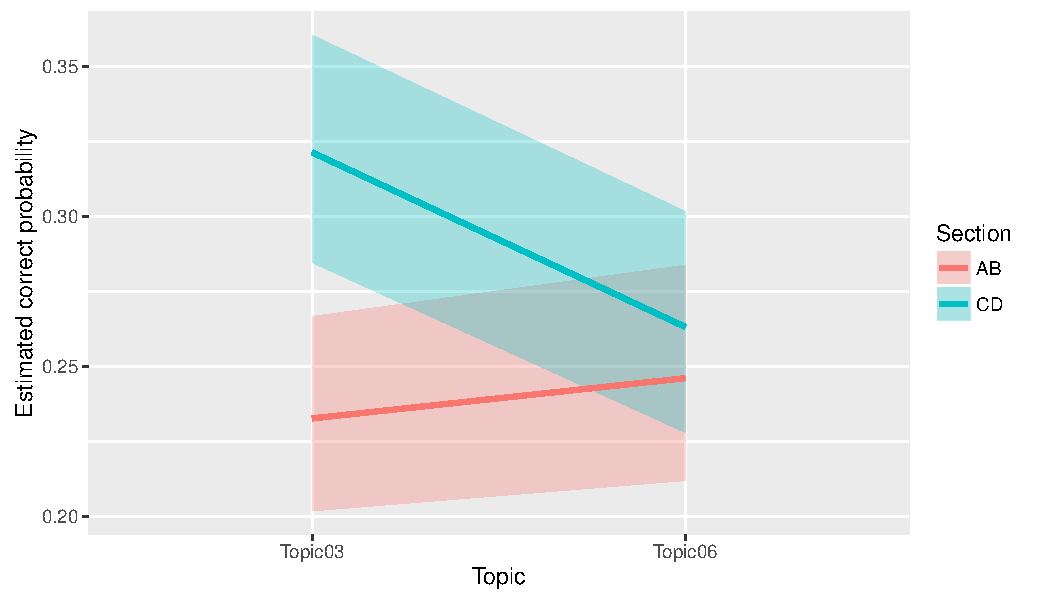
\includegraphics[width=0.95\textwidth]{Stat101_allSections_est_section}
\par\end{centering}
\caption{\label{fig:est_sec}The estimated correct probability by section.
On average, section CD has the highest correct probability, and AB has the lowest.}
\end{wrapfigure}\par\end{center}

\clearpage
From the model we see that some sections are better than other sections,
and some topics are easier to understand than other topics.
So the next question is that are the differences significant
between topics and between sections? 

We run the multiple test for comparison between the topics:
\begin{enumerate}
\item $H_{0}:\;\beta_{t_{i}}=0\qquad\textrm{vs}\qquad H_{a}:\;\beta_{t_{i}}\neq0$\\
for $\forall\; i\in\{2,3,\cdots,$2$\}$.
\item $H_{0}:\;\beta_{t_{i}}-\beta_{t_{j}}=0\qquad\textrm{vs}\qquad H_{a}:\;\beta_{t_{i}}-\beta_{t_{j}}\neq0\qquad$\\
for $\forall\; i\neq j,\; i,j\in\{2,3,\cdots,$2$\}$.
\end{enumerate}
and get the the adjusted p-values by Bonferroni method in Table \ref{tab:pvalues_topic}.

% latex table generated in R 3.2.2 by xtable 1.8-0 package
% Sat Jan 16 13:50:58 2016
{\tiny
\begin{longtable}{rr}
  \hline
 & Topic03 \\ 
  \hline
Topic06 & 0.4085 \\ 
   \hline
\hline
\caption{P-values of the multiple comparison between topics} 
\label{tab:pvalues_topic}
\end{longtable}
}


Then run the multiple test pairwisely between the sections:
\begin{enumerate}
\item $H_{0}:\;\beta_{s_{i}}=0\qquad\textrm{vs}\qquad H_{a}:\;\beta_{s_{i}}\neq0$\\
for $\forall\; i\in\{2,3,\cdots,$2$\}$.
\item $H_{0}:\;\beta_{s_{i}}-\beta_{s_{j}}=0\qquad\textrm{vs}\qquad H_{a}:\;\beta_{s_{i}}-\beta_{s_{j}}\neq0$\\
for $\forall\; i\neq j,\; i,j\in\{2,3,\cdots,$2$\}$.
\end{enumerate}
and get the the adjusted p-values by Bonferroni method in Table \ref{tab:pvalues_sec}.

% latex table generated in R 3.2.2 by xtable 1.8-0 package
% Sat Jan 16 13:50:58 2016
\begin{longtable}{rr}
  \hline
 & AB \\ 
  \hline
CD & 0.0006 \\ 
   \hline
\hline
\caption{P-values of the multiple comparison between sections} 
\label{tab:pvalues_sec}
\end{longtable}



\clearpage
\newpage{}
\section{Clustering}

During a semester of 16 weeks, students may not keep the same pace 
in studying. Some students are smart and working very hard all the 
time. Some students start full of energy, and gradually lose 
their passions. Some students do not take the course seriously 
until they are challenged by some difficult content.

\begin{marginfigure}
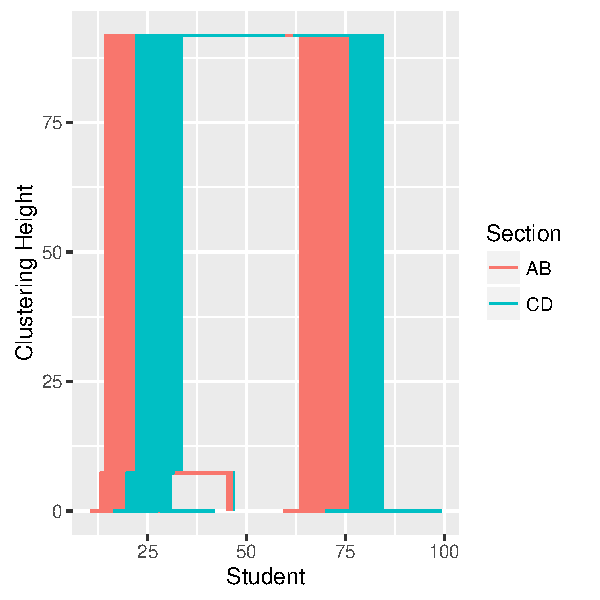
\includegraphics[width=0.98\linewidth]{Stat101_allSections_hclust}
\caption{\label{mar:hclust}Tree plot of hierarchical clustering, 
from one to nine clusters.}
\end{marginfigure}

We are interested in finding some featured behaviors along with time,
by clustering the students into groups. The result of hierarchical 
clustering on the scaled scores is shown in Figure \ref{mar:hclust}. 
Up to down it seperates the students in 1 to 9 groups.
It suggests the best number of clusters is 2.

Note that the euclidean distance of the correct percentages 
is not a reasonable distance measure, because it emphasizes
more on the score level, less on the temporal pattern. 
For example, student A gets 100, 95, 90 for the first three homeworks;
student B gets 70, 65, 60; and student C gets 60, 65, 70.
Student A and B have the same decreasing pattern, but by the 
euclidean distance, B and C are closer.

Similar as using the correlation distance, we scaled the 
correct percentages within the records of each student.
Revisit the example above, the scaled scores for student 
A and B are 1, 0, -1; for student C are -1, 0, 1. Then 
A and B can be grouped together.

\begin{marginfigure}
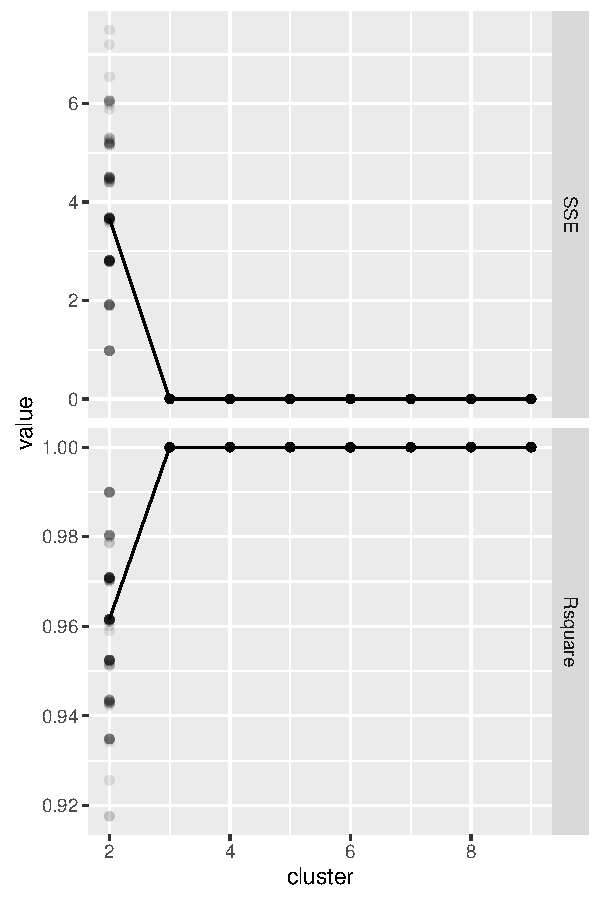
\includegraphics[width=0.98\linewidth]{Stat101_allSections_screeplot}
\caption{\label{mar:scree}Two criteria to refer the number of clusters.
The points are results from bootstrap simulation, and the line connects 
the real values from the criteria.}
\end{marginfigure}

To find the better number of clusters, first we consider two simple 
criteria. One is the within group sum of squares (SSE), the other is 
the proportion of between group sum of squares (SSR) over the total 
sum of squares (SSR+SSE), i.e., the R-square.
Figure \ref{mar:scree} gives the scree plots for SSE and R-squares
for the models with 2 to 9 clusters. The lines connect 
the real values from the criteria, and the dots are the 
bootstrap simulation. The plots suggest 2 clusters.

At the meanwhile, we consider another criterion - the optimum 
average silhouette width. As seen in Figure \ref{mar:asw}, 
it suggests the best number of clusters is 3.

Since 2 clusters is a reasonable choice,
the mean scaled scores of each cluster on each topic is displayed in 
Figure \ref{fig:bestcut}.

\begin{marginfigure}
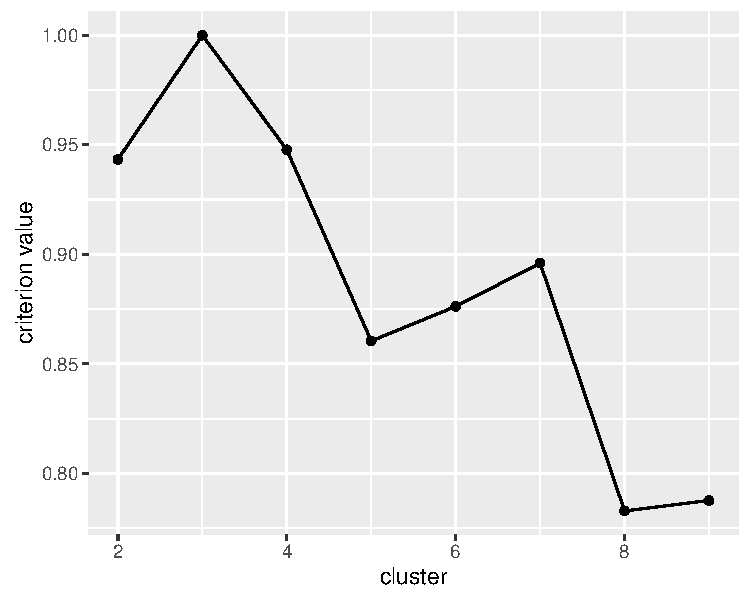
\includegraphics[width=0.98\linewidth]{Stat101_allSections_clustasw}
\caption{\label{mar:asw}Using the optimum average silhouette 
width criterion to find the number of clusters. The larger value, 
the better model.}
\end{marginfigure}% latex table generated in R 3.2.2 by xtable 1.8-0 package
% Sat Jan 16 13:51:07 2016
\begin{longtable}{rrr}
  \hline
 & 1 & 2 \\ 
  \hline
AB & 39.58 & 59.62 \\ 
  CD & 60.42 & 40.38 \\ 
   \hline
\hline
\caption{Contingency table in Column\% between sections and clusters.} 
\label{tab:cluster_pct}
\end{longtable}
\begin{center}
\begin{wrapfigure}{h}{0.95\columnwidth}
\begin{centering}
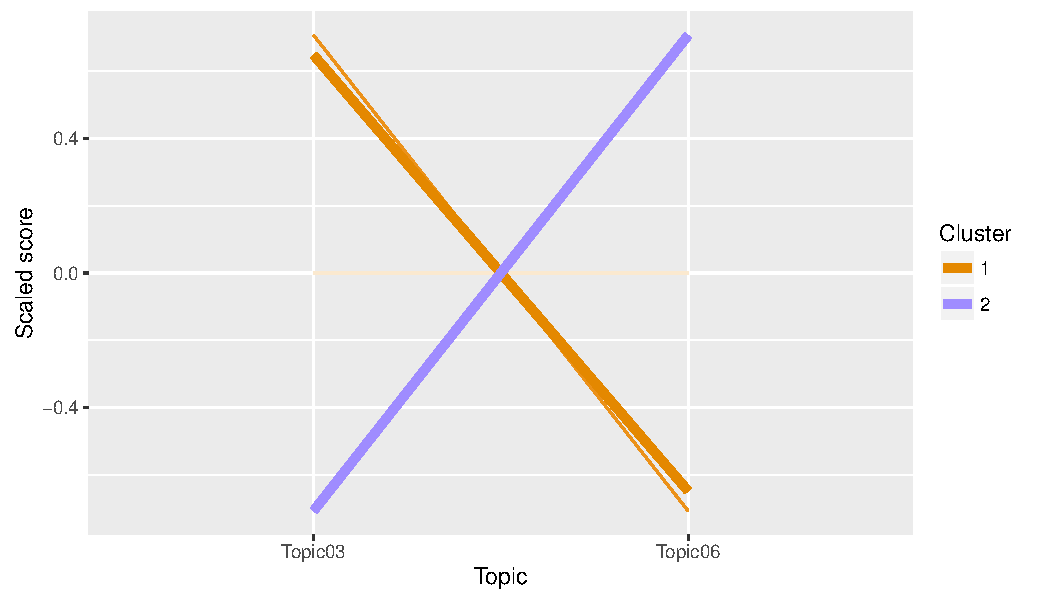
\includegraphics[width=\linewidth]{Stat101_allSections_bestclust}
\par\end{centering}
\caption{\label{fig:bestcut}Trend of the 2 clusters. 
The thick lines connect the means of the clusters; 
the light thin lines show the scaled scores by student.}
\end{wrapfigure}\par\end{center}\begin{marginfigure}
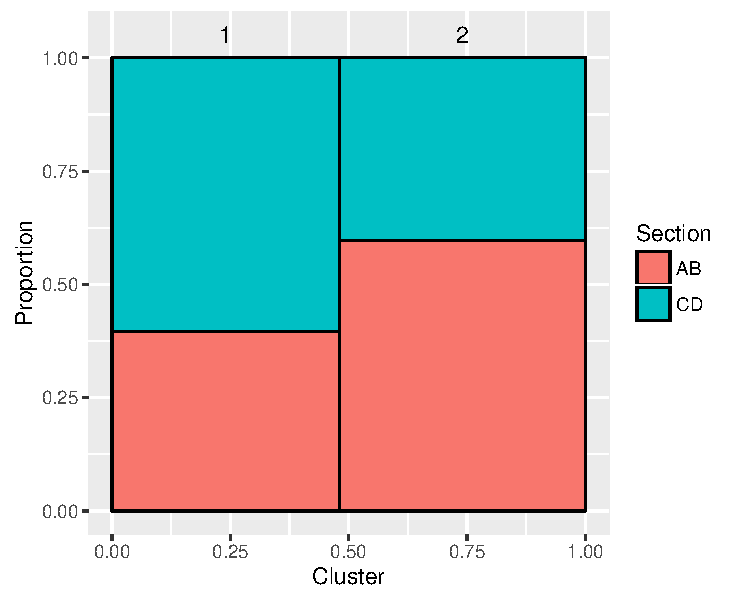
\includegraphics[width=0.98\linewidth]{Stat101_allSections_clust_mosaic}
\caption{\label{mar:mosaic}Mosaic plot by section and cluster.}
\end{marginfigure}

\clearpage
\section{Students}

% latex table generated in R 3.2.2 by xtable 1.8-0 package
% Sat Jan 16 13:51:08 2016
\begin{longtable}{rr}
  \hline
AB & CD \\ 
  \hline
  3 &   0 \\ 
   \hline
\hline
\caption{Number of students that have at least a half of the homework scores in the bottom 20\%.} 
\label{tab:bottom20}
\end{longtable}



\clearpage
\newpage{}
\section{Acknowledgement}
This report is generated by Xiaoyue Cheng, Dianne Cook, Lindsay Rutter, and Amy Froelich, using R-3.1.2 with packages knitr, xtable and ggplot2.

\end{document}
